\documentclass{cvf}
\usepackage{amssymb}

\begin{document}

\chapter{Curriculum Vitae}

\begin{tabular}{c|c}
\begin{minipage}{10cm}
\name{Jorge Alda Gallo}
\vspace{0.8cm}
\presentation{Ph.D. in Theoretical Physics}
\noindent
\email{jorge.alda@pd.infn.it}
\phone{+34 676 70 35 11}
\address{via Ognissanti 81 int 2. 35129 Padova (PD), Italy}
\webpage{https://jorge-alda.github.io}
\github{Jorge-Alda}
\orcid{0000-0002-6728-1105} 
\end{minipage} & \hspace{1cm} 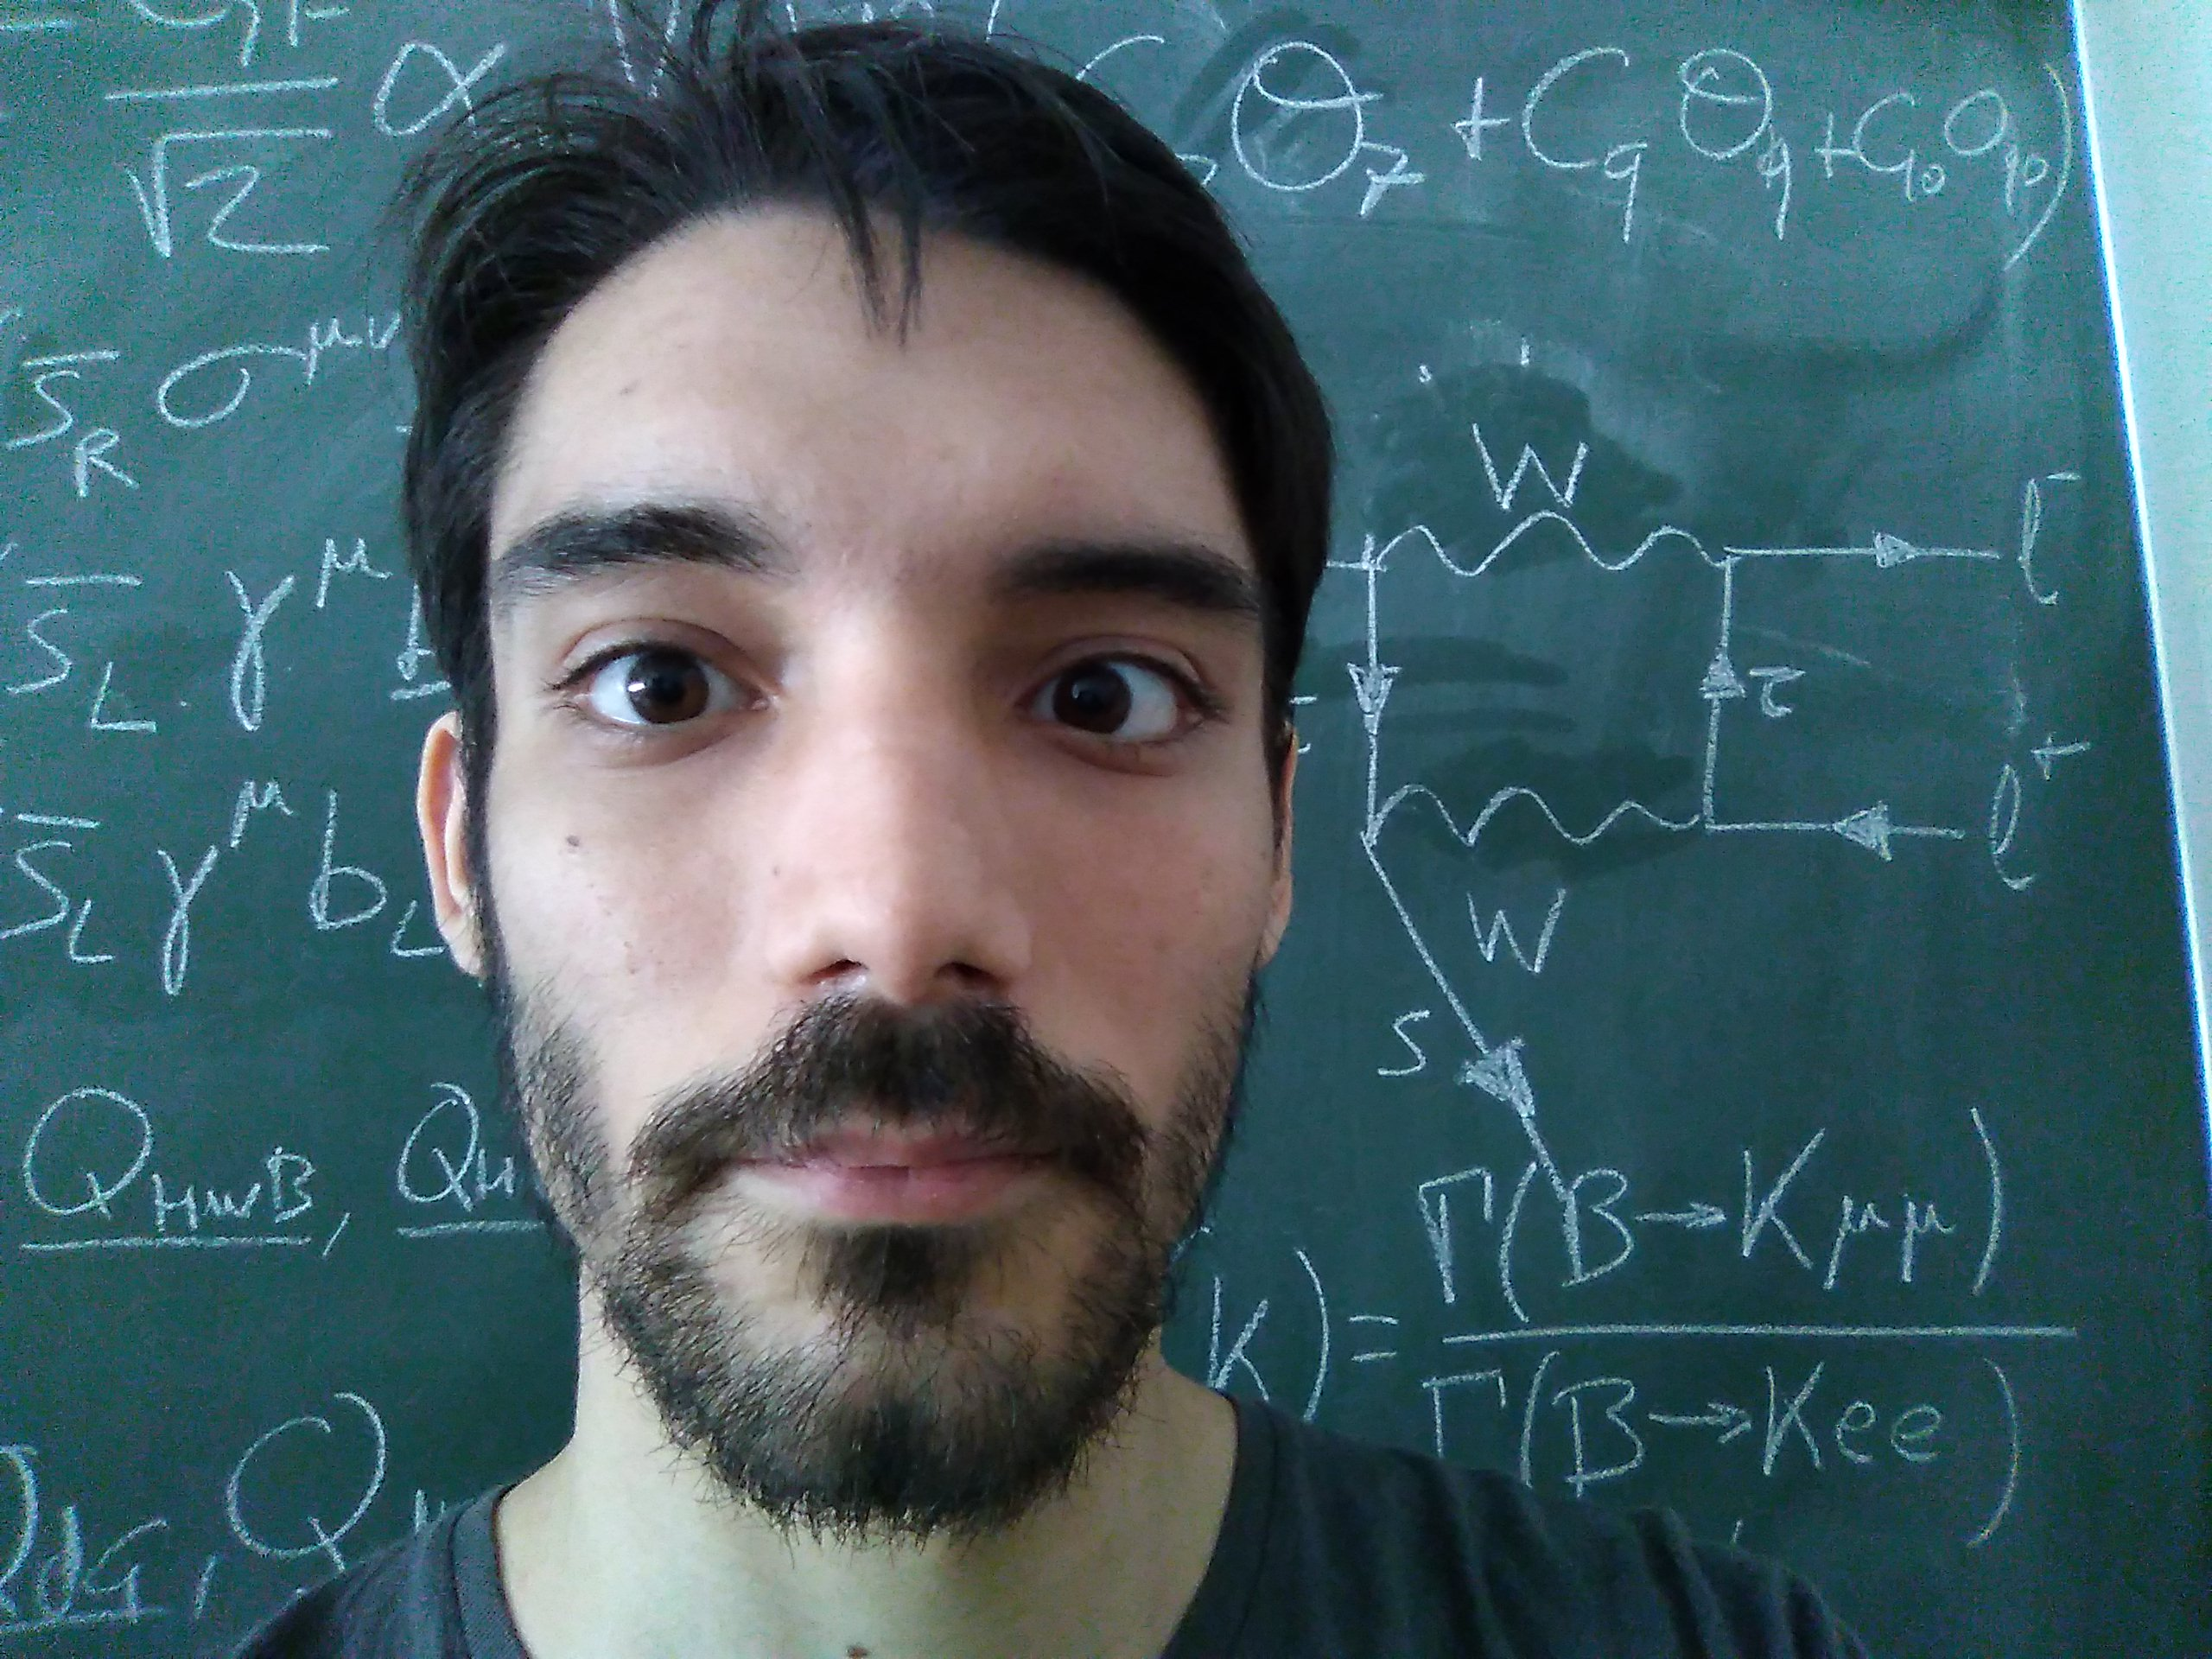
\includegraphics[width=4cm]{photo.jpg}
\end{tabular}

\interests{Research interests}
\begin{itemize}
\item New physics beyond the Standard Model.
\item Flavour Physics.
\item $B$-meson anomalies.
\item Effective Field Theories.
\item Axions and Axion-like particles.
\item Machine Learning applied to Physics.
\end{itemize}

\education{Education}
\datedsubsection{B.Sc. in Physics, Universidad de Zaragoza}{2011-2015}
Average grade: 9.20/10. 13 Honours.\\
B.Ss. Project: \textit{``Cálculo numérico en teoría cuántica de campos de la materia condensada''}. Under the supervision of David Zueco Láinez. Qualification: 9.5/10.

\datedsubsection{M.Sc. in Theoretical Physics, Universidad Complutense de Madrid}{2015-2016}
Average grade: 9.34/10.\\
M.Sc. Project: \textit{New Applications of the Coleman-Weinberg Model}. Under the supervision of J. A. Ruiz Cembranos. Qualification: 9.0/10.

\datedsubsection{Ph.D. in Physics, Universidad de Zaragoza}{2016-2022}
Under the supervision of Siannah Peñaranda Rivas.\\
Dissertation title: \textit{A Glance into Flavour Physics with Effective Field Theories and Machine Learning}.\\
Defense date: 27th April 2022.\\
Qualification: \textit{Cum Laude}.

\datedsubsection{Ph.D. School}{2018}
Taller de Altas Energías. Benasque (Huesca, Spain).

\datedsubsection{Ph.D. School}{2022}
WE-Heraeus Summer School SMEFT'22: Theory and Phenomenology of the Standard Model EFT. Siegen (Germany).

\invited{Positions}

\datedsubsection{Universidad de Zaragoza}{April 2022 - February 2023}

\datedsubsection{Università degli Studi di Padova}{October 2023 - September 2025}


\datedsubsection{Università degli Studi di Padova}{December 2025 - December 2027}
Contratto di Ricerca.

\grants{Grants}
\datedsubsection{Grant JAE-Intro CSIC}{2014}
Project \textit{``Caos semiclásico en sistemas de bosones con interacción''}, supervised by David Zueco Láinez.\\
CSIC-ICMA (Spanish National Research Council and Instituto de Ciencia de Materiales de Aragón).

\datedsubsection{PreDoc Grant, Diputación General de Aragón}{2017-2022}

\datedsubsection{Programa Ibercaja-CAI de Estancias de Investigación}{2021}
Grant No. CB 5/21.

\datedsubsection{Postdoctoral Scholarship for Extension of Studies Abroad for Life and Material Sciences, Ramón Areces Foundation}{2023-2025}

\memberships{Memberships}
\datedsubsection{CAPA}{2019-present}
Centro de Astropartículas y Física de Altas Energías. Zaragoza, Spain.\\
\url{capa.unizar.es}

\datedsubsection{INFN}{2023-present}
Associated to Istituto Nazionale di Fisica Nucleare, Sezione di Padova.

\datedsubsection{COMCHA}{2026-2028}
Spanish Network on Advanced Computing for Fundamental and Applied Physics.\\
Convener of WG2: Simulation and Modelling.

\invited{Visiting Scholar Appointments}
\datedsubsection{Università degli Studi di Padova/INFN}{Summer 2021}

\datedsubsection{Università degli Studi di Padova/INFN}{Summer 2023}

\datedsubsection{University of California, San Diego}{September 2024}

\datedsubsection{Laboratori Nazionali del Gran Sasso}{November 2024}

\datedsubsection{Kavli IPMU, Tokyo}{May-June 2026}

\works{Scientific Production}

\hspace{\parindent}
\textbf{J. Alda, J. Guasch and S. Peñaranda: \textit{Some results on Lepton Flavour Universality Violation}}\\
Eur.Phys. J. C, 79 7 (2019) 588\\
doi:\href{https://doi.org/10.1140/epjc/s10052-019-7092-x}{10.1140/epjc/s10052-019-7092-x}\\
arXiv:\href{https://arxiv.org/abs/1805.03636}{1805.03636 [hep-ph]}

~

\textbf{J. Alda, J. Guasch and S. Peñaranda: \textit{Anomalies in $B$ decays: A phenomenological approach}}\\
Eur.Phys. J. Plus 137 (2022) 217\\
doi:\href{https://doi.org/10.1140/epjp/s13360-022-02405-3}{10.1140/epjp/s13360-022-02405-3}\\
arXiv:\href{https://arxiv.org/abs/2012.14799}{2012.14799 [hep-ph]}

~

\textbf{J. Alda, J. Guasch and S. Peñaranda: \textit{Anomalies in $B$ decays: Present status and future collider prospects}}\\
arXiv:\href{https://arxiv.org/abs/2105.05095}{2105.05095 [hep-ph]}\\
SLAC eConf C21-03-15.1

~

\textbf{J. Alda, J. Guasch and S. Peñaranda: \textit{Using Machine Learning techniques in phenomenological studies in flavour physics}}\\
J. High Energ. Phys. 2022, 115 (2022)\\
doi:\href{https://doi.org/10.1007/JHEP07(2022)115}{10.1007/JHEP07(2022)115}\\
arXiv:\href{https://arxiv.org/abs/2109.07405}{2109.07405 [he-ph]}

~

\textbf{J. Alda, J. Guasch and S. Peñaranda: \textit{Exploring B-physics anomalies at colliders}}\\
arXiv:\href{https://arxiv.org/abs/2110.12240}{2110.12240 [hep-ph]}\\
PoS(EPS-HEP2021)494

~

\textbf{J. Alda, A. W. M Guerrera, S. Peñaranda and S. Rigolin: \textit{Leptonic Meson Decays into Invisible ALP}}\\
Nucl.Phys.B 979 (2022) 115791\\
doi:\href{https://doi.org/10.1016/j.nuclphysb.2022.115791}{10.1016/j.nuclphysb.2022.115791}\\
arXiv:\href{https://arxiv.org/abs/2111.02536}{2111.02536 [hep-ph]}

~

\textbf{J. Alda, G. Levati, P. Paradisi, S. Rigolin and N. Selimovi\'c: \textit{Collider and astrophysical signatures of light scalars with enhanced $\tau$ couplings}}\\
JHEP 06 (2025) 008\\
doi:\href{https://doi.org/10.1007/JHEP06(2025)008}{10.1007/JHEP06(2025)008}\\
arXiv:\href{https://arxiv.org/abs/2407.18296}{2407.18296 [hep-ph]}\\

~

\textbf{J. Alda, A. Mir and S. Peñaranda: \textit{Flavour anomalies and Machine Learning: an improved analysis}}\\
Int.J.Theor.Phys. 65 (2026) 2, 46\\
doi:\href{https://doi.org/10.1007/s10773-026-06263-y}{10.1007/s10773-026-06263-y}\\
arXiv:\href{https://arxiv.org/abs/2412.15830}{2412.15830 [hep-ph]}\\


~

\textbf{J. Alda, C. Broggini, G. Di Carlo, L. Di Luzio, D. Piatti, S. Rigolin and C. Toni: \textit{Time modulation of weak nuclear decays as a probe of axion dark matter}}\\
Phys.Rev.D 111 (2025) 3, 035022\\
doi:\href{https://doi.org/10.1103/PhysRevD.111.035022}{10.1103/PhysRevD.111.035022}\\
arXiv:\href{https://arxiv.org/abs/2412.20932}{2412.20932 [hep-ph]}\\


~

\textbf{J. Alda, M. Fuentes Zamoro, L. Merlo, X. Ponce D{\'\i}az and S. Rigolin: \textit{Comprehensive ALP Searches in Meson Decays}}\\
arXiv:\href{https://arxiv.org/abs/2507.19578}{2507.19578 [hep-ph]}\\
Submitted to Fortschritte der Physik

~

\textbf{J. Alda, M. Fuentes Zamoro, L. Merlo, X. Ponce D{\'\i}az and S. Rigolin: \textit{Comprehensive ALP Searches in Meson Decays}}\\
arXiv:\href{https://arxiv.org/abs/2508.08354}{2508.08354 [hep-ph]}\\
Submitted to Computer Physics Communications

~

\textbf{A. Mir, J. Alda and S. Peñaranda: \textit{B-Meson Anomalies: Effective Field Theory Meets Machine Learning}}\\
arXiv:\href{https://arxiv.org/abs/2510.17742}{2510.17742 [hep-ph]}\\
Contribution to EPS-HEP2025

~

\textbf{M. Fuentes Zamoro, J. Alda, L. Merlo, X. Ponce D{\'\i}az and S. Rigolin: \textit{Tackling ALP searches in meson decays with ALPaca: a phenomenological approach}}\\
Proceedings of 3rd General Meeting of the COST Action COSMIC WISPers (CA21106)\\
\url{https://pos.sissa.it/507/057}

~

\textbf{J. Alda: \textit{Lecture notes on Machine Learning applications for global fits}}\\
arXiv:\href{https://arxiv.org/abs/2604.07520}{2604.07520 [hep-ph]}\\
Submitted to SciPotst Physics Lectures Notes

~

\textbf{J. Alda, J. Asorey, A. Mir, S. Peñaranda: \textit{Physically Consistent Parameter Inference: Transparent Machine Learning Emulation in High Energy Physics and Cosmology}}\\
arXiv:\href{https://arxiv.org/abs/2607.12726}{2607.12726 [hep-ph]}\\
Submitted to Universe (Invited contribution to Special Issue ``Advances in Machine Learning Techniques in Cosmology and Particle Physics'')

~

\textbf{J. Alda, L. C. Bresciani, G. Levati, P. Paradisi, S. Rigolin and N. Selimovi\'c: \textit{Leptonic Couplings of Axion-Like Particles: Constraints from Present and Next-Generation Colliders}}\\
In preparation

~

\textbf{J. Alda, S. Rigolin: \textit{ALPs in Chiral Perturbation Theory: general framework and baryon interactions}}\\
In preparation


\conferences{Talks and conferences}

\hspace{\parindent}\textbf{2nd Red LHC Workshop. Madrid, Spain. 9-11 May 2018}\\
Talk ``Some Results on Lepton Flavour Violation''.

~

\textbf{Taller de Altas Energías. Benasque (Huesca, Spain) 2-15 September 2018}\\
Talk ``Some Results on Lepton Flavour Violation''.

~

\textbf{X CPAN Days. Salamanca, Spain. 29-31 October 2018}\\
Talk ``Complex Wilson coefficients in the analysis of $B$-anomalies''.

~

\textbf{I Jornadas de Jóvenes Investigadores CAPA. Zaragoza, Spain. 7 May 2019}\\
Invited Talk ``Effective Theories for $B$-meson anomalies''.

~

\textbf{I Jornadas del Programa de Doctorado de Física. Zaragoza, Spain. 20 June 2019}\\
Invited Talk ``Effective Theories for $B$-meson anomalies''.

~

\textbf{XXXVII Bienal de Física de la Real Sociedad Española de Física. Zaragoza, Spain. 15-19 de July 2019}\\
Talk ``Some Results on Lepton Flavour Universality Violation''.

~

\textbf{International Workshop on Future Linear Colliders - LCWS2021. Online. 15-18 March 2021}\\
Talk ``Anomalies in $B$ mesons decays: Present status and future collider prospects''.

~

\textbf{European Physical Society Conference on High Energy Physics 2021 (EPS-HEP2021). Online. 26-30 July 2021}\\
Poster ``Exploring B-physics anomalies at colliders ''.

~

\textbf{Seminar, Department of Theoretical Physics. University of Zaragoza, Spain. 18 November 2021}\\
Invited Talk ``Leptonic Mesons Decays into invisible ALP''.

~

\textbf{II Jornadas del Programa de Doctorado de Física. University of Zaragoza, Spain. 3 December 2021}\\
Invited Talk ``Leptonic Mesons Decays into invisible ALP''.

~

\textbf{Seminar, Department of Theoretical Physics. University of Zaragoza, Spain. 20 January 2022}\\
Invited Talk ``Using Machine Learning techniques in phenomenological studies in flavour physics''.

~

\textbf{Seminar, Institute of Theoretical Physics (IFT). Autonomous University of Madrid, Spain. 27 January 2022}\\
Invited Talk ``Using Machine Learning techniques in phenomenological studies in flavour physics''.

~

\textbf{XIII CPAN Days. Huelva, Spain. 21-23 March 2022}\\
Talk ``Using Machine Learning techniques in phenomenological studies in flavour physics''.

~

\textbf{5th Inter-experiment Machine Learning Workshop. CERN, Switzerland. 8-13 May 2022}\\
Talk ``Using Machine Learning techniques in phenomenological studies in flavour physics''.

~

\textbf{Saturnalia Workshop. University de Zaragoza/CAPA, Spain. 21 December 2022}\\
Invited Talk ``Using Machine Learning techniques in phenomenological studies in flavour physics''.

~

\textbf{Saturnalia Workshop. University de Zaragoza/CAPA, Spain. 20 December 2023}\\
Invited Talk ``Light New Physics coupling to $\tau$''.

~

\textbf{Seminar, Institute of Theoretical Physics (IFT). Autonomous University of Madrid, Spain. 06 June 2024}\\
Invited Talk ``Leptophilic Axion-Like Particles''.

~

\textbf{Seminar, University of California, San Diego. 17 September 2024}\\
Invited Talk ``Signatures of light scalars with enhanced $\tau$ couplings''.

~

\textbf{Flavour for New Physics at Present and Future Colliders Workshop. Mainz Institute for Theoretical Physics, Johannes Gutenberg University, Germany. 19 June 2025}\\
Invited Talk ``Present and future of ALP searches in colliders''.

~

\textbf{Invisibles25 Workshop. CERN, Switzerland. 4 September 2025}\\
Talk ``ALP searches in meson decays with ALPaca: a phenomenological approach''.

~

\textbf{Implications of LHCb measurements and future prospects. CERN, Switzerland. 5 November 2025}\\
Invited Talk ``ALP searches in meson decays with ALPaca''.

~

\textbf{Saturnalia Workshop. University de Zaragoza/CAPA, Spain. 18 December 2025}\\
Invited Talk ``GeV-ALP searches with ALP-aca''.

~

\textbf{4th COMCHA School. University of Zaragoza/CAPA, Spain. 14 April 2026}\\
Invited Talk and hands-on session ``ML for global fits''.

~

\textbf{Invisibles26 Workshop. A Coru\~na, Spain. 10-14 August 2026}\\
Poster ``GeV ALP interactions with hadrons''.

\repositories{Contributions to public repositories}

\subsection{flavio}
1 pull request merged: \url{https://github.com/flav-io/flavio/pull/160}

\subsection{smelli}
1 pull request: \url{https://github.com/smelli/smelli/pull/45}

\subsection{ALP Automatic Computing Algorithm (ALP-aca)}
Main contributor. \url{https://github.com/alp-aca}

Open source Python library for the phenomenology of Axion-Like Particles (ALPs) in meson decays. It provides a framework to match from specific UV models, run the RGE equations, compute the branching ratios of meson decays into ALPs and the corresponding experimental constraints, and set exclusion regions.

\teaching{Teaching}

\subsection{September 2019}
\hspace{\parindent}\textbf{Ph.D. School ``Taller de Altas Energías de Benasque'' (Huesca, Spain).}\\
Associate teacher.

\subsection{2019-2020}
\hspace{\parindent}\textbf{Differential Equations}\\
Problem-solving sessions, 38 teaching hours.\\
Second year course, Bachelor Degree in Physics, Universidad de Zaragoza.

~

\textbf{General Physics}\\
Laboratory sessions, 10 teaching hours.\\
First year course, Bachelor Degree in Mathematics, Universidad de Zaragoza.

\subsection{2020-2021}
\hspace{\parindent}\textbf{Differential Equations}\\
Problem-solving sessions, 38 teaching hours.\\
Second year course, Bachelor Degree in Physics, Universidad de Zaragoza.

~

\textbf{General Physics}\\
Laboratory sessions, 10 teaching hours.\\
First year course, Bachelor Degree in Mathematics, Universidad de Zaragoza.

\subsection{2021-2022}
\hspace{\parindent}\textbf{Differential Equations}\\
Problem-solving sessions, 38 teaching hours.\\
Second year course, Bachelor Degree in Physics, Universidad de Zaragoza.

~

\textbf{Co-direction of B.Sc. Project: Alejandro Mir}\\
10 teaching hours.
Fourth year course, Bachelor Degree in Physics, Universidad de Zaragoza.

~

\textbf{General Physics}\\
Laboratory sessions, 10 teaching hours.\\
First year course, Bachelor Degree in Mathematics, Universidad de Zaragoza.

\subsection{2022-23}
\hspace{\parindent}\textbf{Co-direction of M.Sc. Project: Alejandro Mir}\\
10 teaching hours.
Master Degree in Physics, Universidad de Zaragoza.

~

\textbf{Co-direction of B.Sc. Project: Francisco J. Gómez-Fauro}\\
10 teaching hours.
Fourth year course, Bachelor Degree in Physics, Universidad de Zaragoza.

\subsection{2024-present}
~

\textbf{Co-direction of Ph.D. Thesis: Alejandro Mir}\\
Co-direction of Ph.D. Thesis in Physics, Universidad de Zaragoza.

\subsection{September 2026}
~
\textbf{Co-direction of Master Thesis: Filippo Cucchetto}\\
Co-direction of Master Thesis in Physics, Università degli Studi di Padova.

\dissemination{Scientific Dissemination}
\textbf{Dark Matter Day. University of Zaragoza, Spain. 31 October 2022}

~

\textbf{Organizing Committee of the 2022 Saturnalia Workshop. University of Zaragoza/CAPA, Spain. 16-22 December 2022}\\
\url{https://indico.capa.unizar.es/event/32/}

~

\textbf{Local Organizing Comitte of PLANCK2025 - The 27th International Conference From the Planck Scale to the Electroweak Scale. Padova, Italy. 26-30 May 2025}\\
\url{https://indico.dfa.unipd.it/event/1200/}

~

\textbf{4th Training School on Computing Challenges, COMCHA network. University of Zaragoza/CAPA, Spain. 8-15 April 2026}\\
\url{https://indico.capa.unizar.es/event/42/}\\
Topical lecture and hands-on session ``ML for global fits''.

~

\textbf{Junior Organizing Comittee of Invisibles26. A Coru\~na, Spain, 10-14 August 2026}\\
\url{https://indico.cern.ch/event/1561367/}

\languages{Languages}
\begin{tabular}{ll}
Spanish & \level{5} \\
English & \level{5} \\
Italian & \level{4} [C1 certification] \\
German & \level{3} \\
French & \level{2}
\end{tabular}

\coding{Programming languages}
\begin{tabular}{ll}
\TeX/\LaTeX & \level{5}\\
Python & \level{5}\\
C/C++ & \level{3}\\
Mathematica & \level{3} \\
Docker & \level{2} \\
Rust & \level{1}
\end{tabular}

\awards{Awards}
\datedsubsection{XXII Spanish Physics Olympiad}{2011}
Silver Medal (Rank 15).\\
Second position in the regional Aragonese phase.

\datedsubsection{20th International Mathematics Competition}{2013}
Bronze Medal (rank 177).

\newpage

\section{About this CV}
\begin{tabular}{L{10.5cm}C{5.5cm}}
\begin{minipage}[b]{10cm}
This CV was last updated in \today.\\
You can find the latest version at \\ \url{https://github.com/Jorge-Alda/Jorge-Alda/releases/latest/download/CV.pdf}
\end{minipage} & 
\includegraphics[width=3cm]{qrcode.png}
\end{tabular}


\end{document}